\section{Design} \label{designsection}

\begin{figure}[htbp]
\centering
\fbox{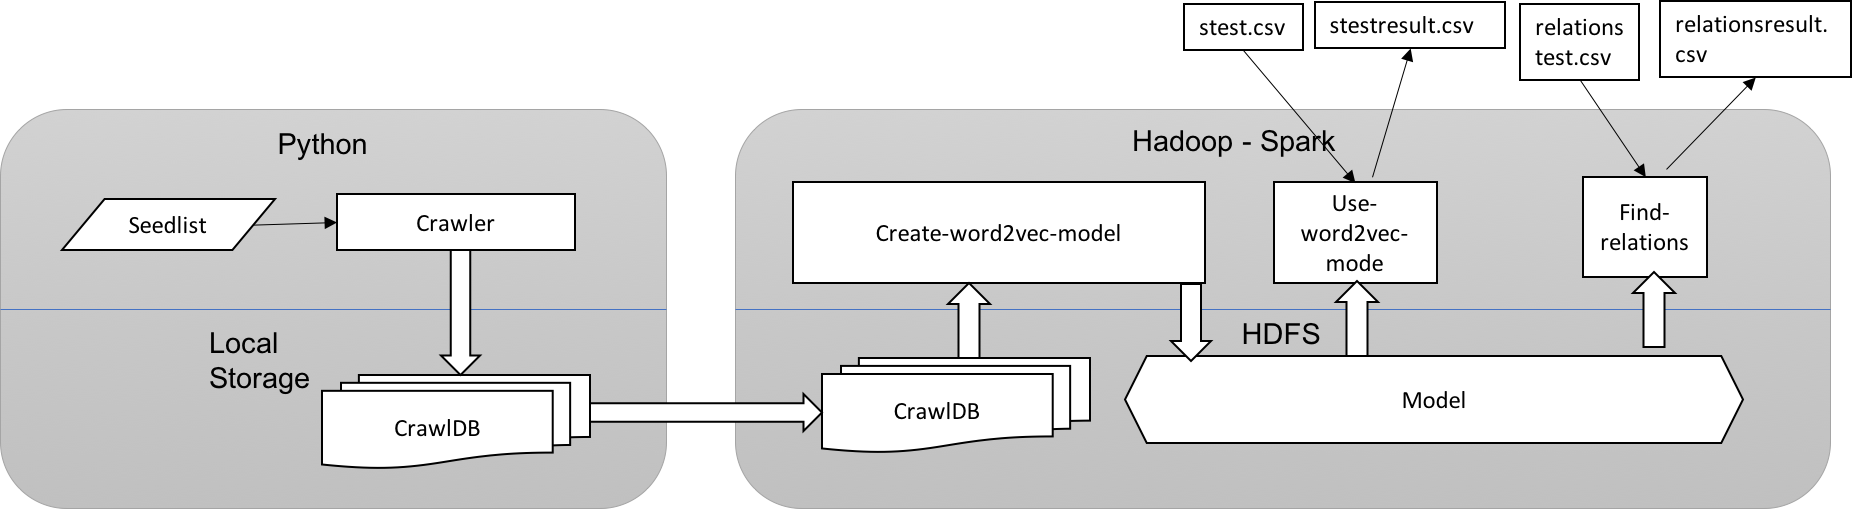
\includegraphics[width=\linewidth]{images/datapipeline.png}}
\caption{Data Pipeline.}
\label{fig:datapipeline}
\end{figure}

Figure \ref{fig:datapipeline} shows the overall data pipeline for the
project. The data pipeline has three important stages:
\begin{itemize}
\item Crawler: Crawler runs in batch mode on a standalone machine. It can
download wikipedia data as explained in section \ref{crawlersection}. Crawler
 creates CrawlDB which is a collection of text files. This crawler can be
 replaced or augmented with any web-crawler which can download or create the
 text files.

\item create-word2vec-model: This component is responsible for creating the
word2vec model for the text files in the CrawlDB. This model runs on Spark
and stores the model on HDFS. Section \ref{createmodelsection} describes this
 component in detail.

\item use-word2vec-model and find-relations: These two components use the
precreated word2vec model to find synonym of a word or find the relationships.
Section \ref{usemodel} describes these components in detail.
\end{itemize}

\subsection{Crawler} \label{crawlersection}
The Crawler component is useful to download the data from web. We implemented
 a simple crawler using Python which can deep traverse the wikipedia pages
 and download the text from it. In our crawler implementation, a user can
 specify the seed pages from wikipedia. User can also specify the maximum
 number of pages that are required to be downloaded. The crawler first
 downloads all the pages specified in the seedlist. It then extract the links
  from each wikipedia page and puts it in a queue which is internally
  maintained by the crawler. The crawler then downloads the the linked pages.
   Since this logic is implemented in recursive manner, the crawler can
   potentially download all the wikipedia pages which can be reached from the
   pages in the seedlist.

    We followed the seedlist based crawler approach so that we can retrieve
    domain specific web pages. A well chosen seedlist can fetch large number
    of relevant web pages.

 Figure \ref{fig:crawleralgo} is the flowchart of the crawler implementation.
\begin{figure}[htbp]
\centering
\fbox{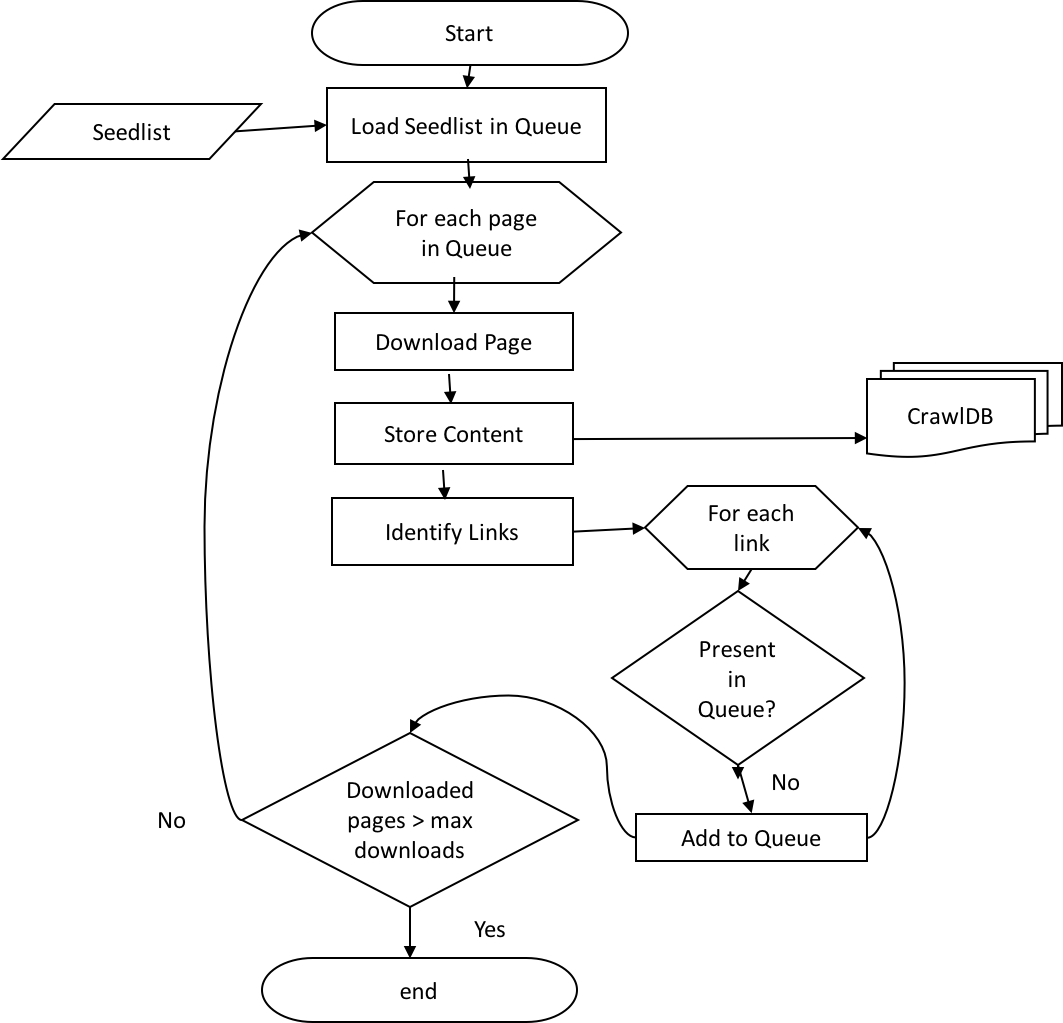
\includegraphics[width=\linewidth]{images/crawleralgo.png}}
\caption{Flowchart of crawler.}
\label{fig:crawleralgo}
\end{figure}

\subsection{Word2Vec Model Creation} \label{createmodelsection}


\subsection{Using the Word2Vec Model} \label{usemodel}


